\documentclass[]{article}

\usepackage{ngerman}
\usepackage{comment}
\usepackage[ngerman]{babel}
\usepackage[utf8]{inputenc}
\usepackage[T1]{fontenc}
\usepackage{amsmath}
\usepackage{graphicx}
\usepackage{caption}
\usepackage{subcaption}
\usepackage{float}


% Title Page
\title{3D Vision LU}
\author{Christian Br\"andle \\
\texttt{Matr.Nr.: 1428543}
\and Stefan Zaufl \\
\texttt{ Matr.Nr.: 0925357}
\and Dominik Sch\"orkhuber\\
\texttt{ Matr.Nr.: 1027470}}

\begin{document}

\maketitle

%\begin{abstract}
%\end{abstract}

\section{Einleitung}  % dominik
In dieser Übung wurden von uns selbst gewählte Objekte mit einem 3D-Laserscanner virtualisiert. Dieses Dokument enthält alle Schritte des Scan- und Bearbeitungsvorganges. Eine abschließende Evaluation und ein Vergleich mit Autodesk 123D Catch zeigt die Qualität und Genauigkeit der erzeugten Modelle. 

\section{Modelle}
\subsection{Budha}

Das Modell von Christian Brändle ist eine kleine Budhastatue - siehe Abbildung \ref{fig:budha_org}.
\begin{figure}[H]
\caption{Budha}
\centering
\includegraphics[scale=0.4]{images/Budha/Budha_Original.jpg}
\label{fig:budha_org}
\end{figure}

\subsection{Mann}
Das Modell von Stefan Zaufl ist eine Statuette von einem zusammengekauertern, weinenden Mann. Zu sehen in Abbildung \ref{fig:man:orig}.
\begin{figure}[H]
\caption{Weinender Mann}
\centering
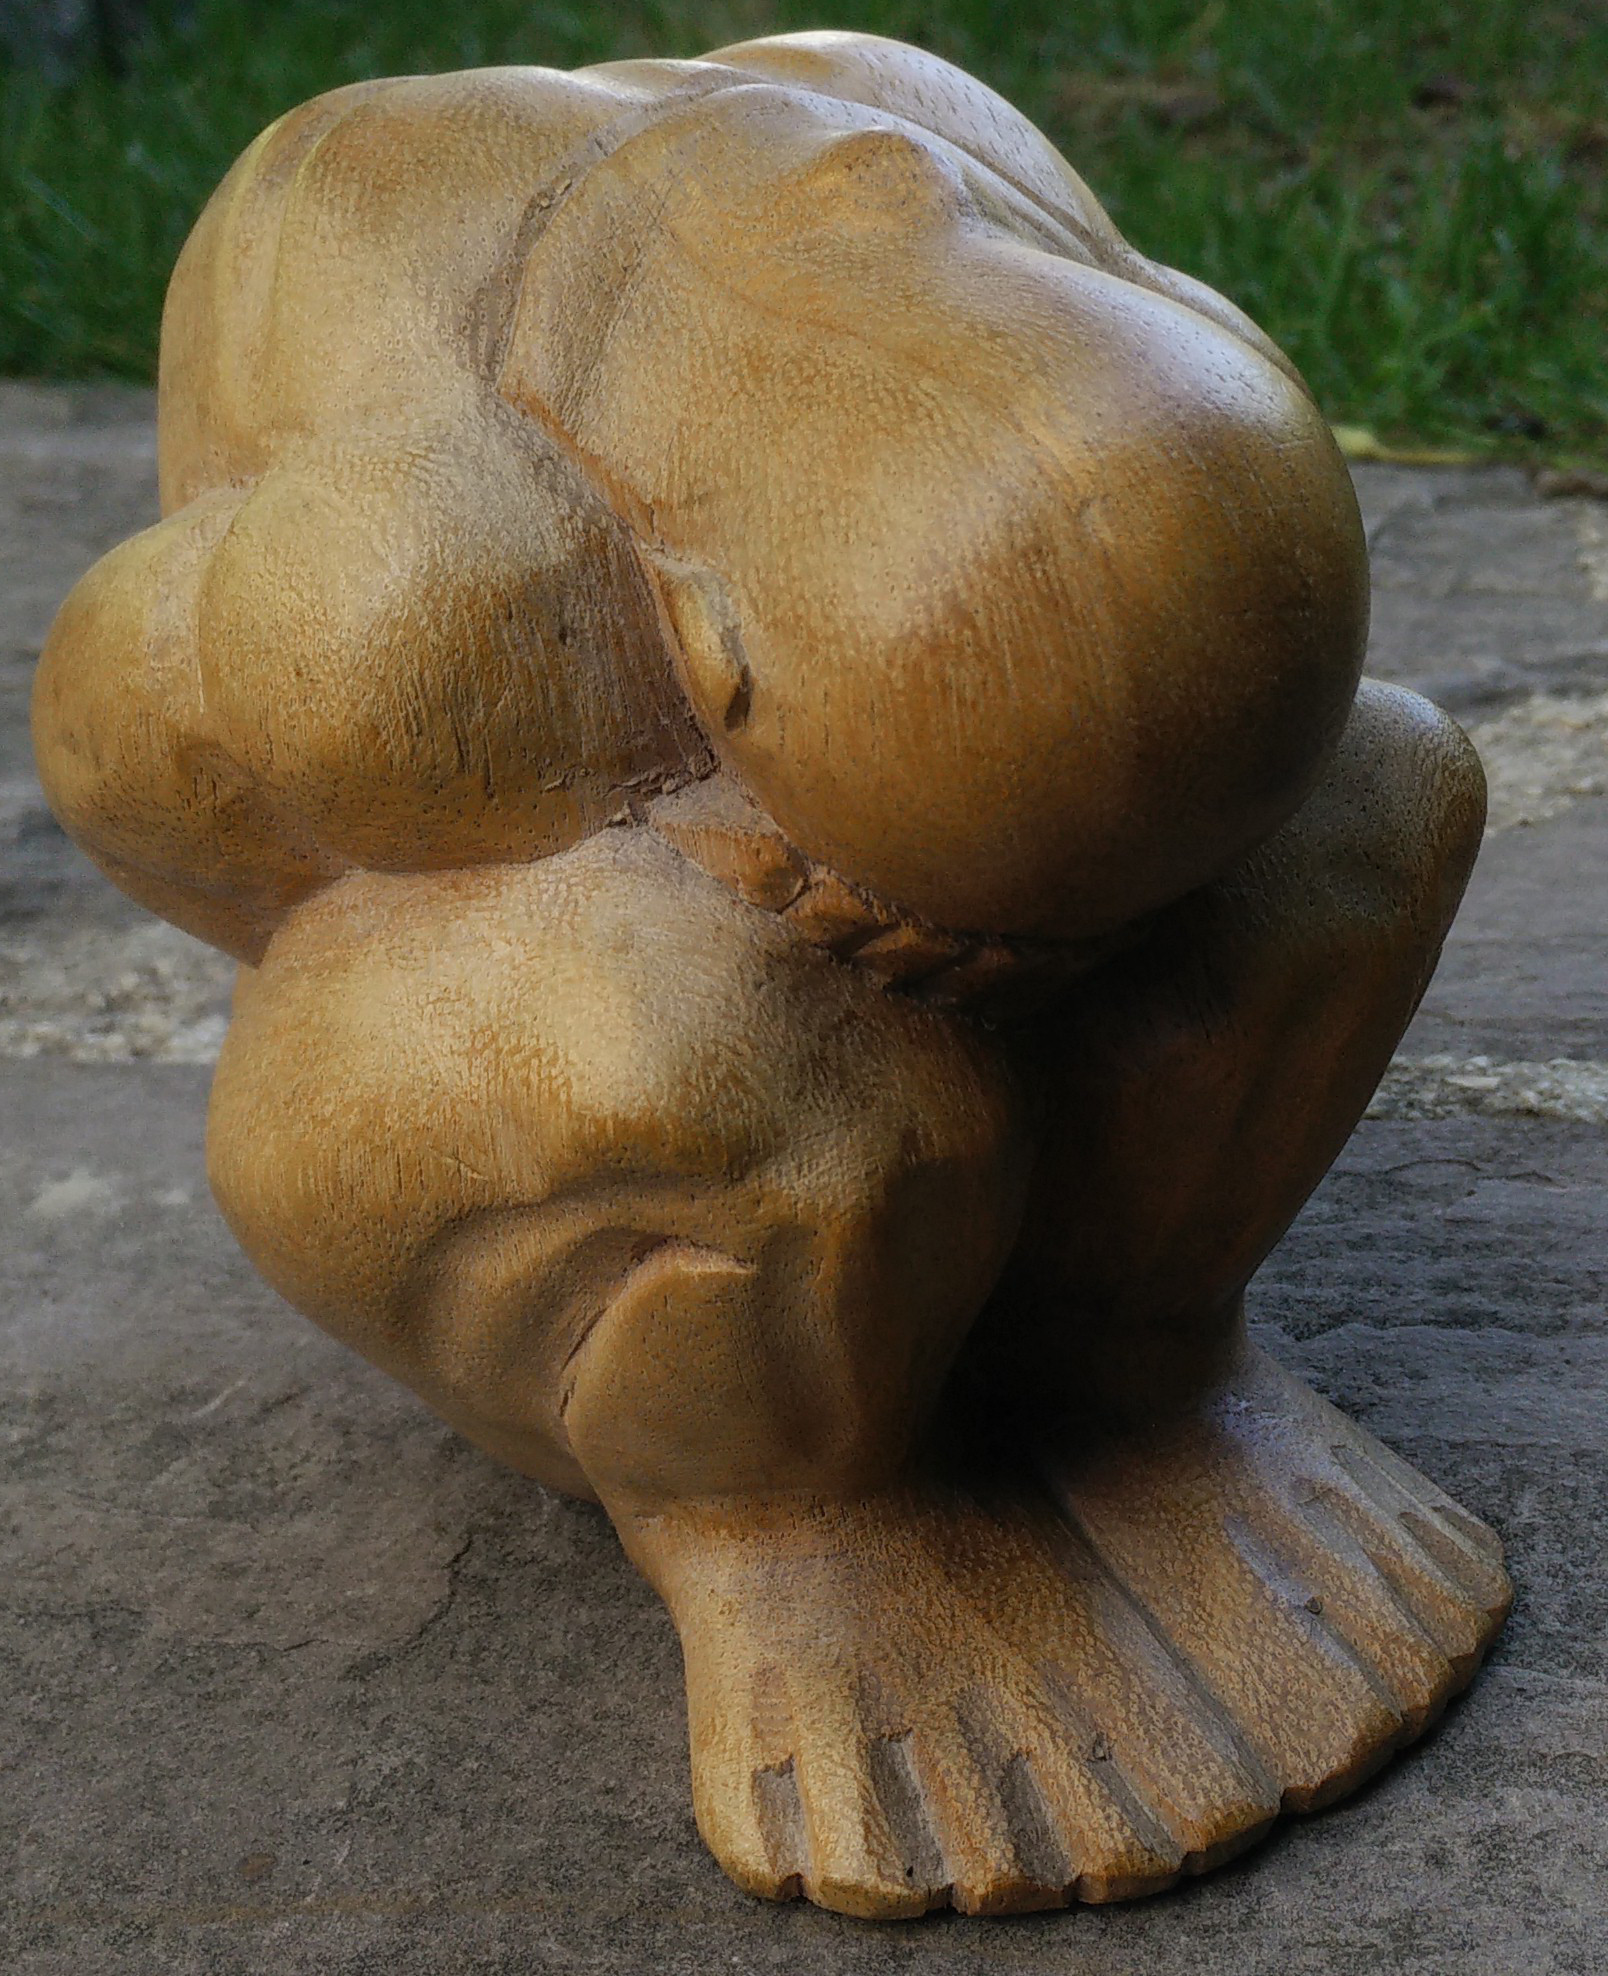
\includegraphics[scale=0.11]{images/Mann_Original.jpg}
\label{fig:man:orig}
\end{figure}


\subsection{Sparschwein}
Das Modell von Dominik Schörkhuber ist das Schwarzgeld Sparschwein. Zu sehen in Abbildung \ref{fig:piggy}.
\begin{figure}[H]
\caption{Sparschwein}
\centering
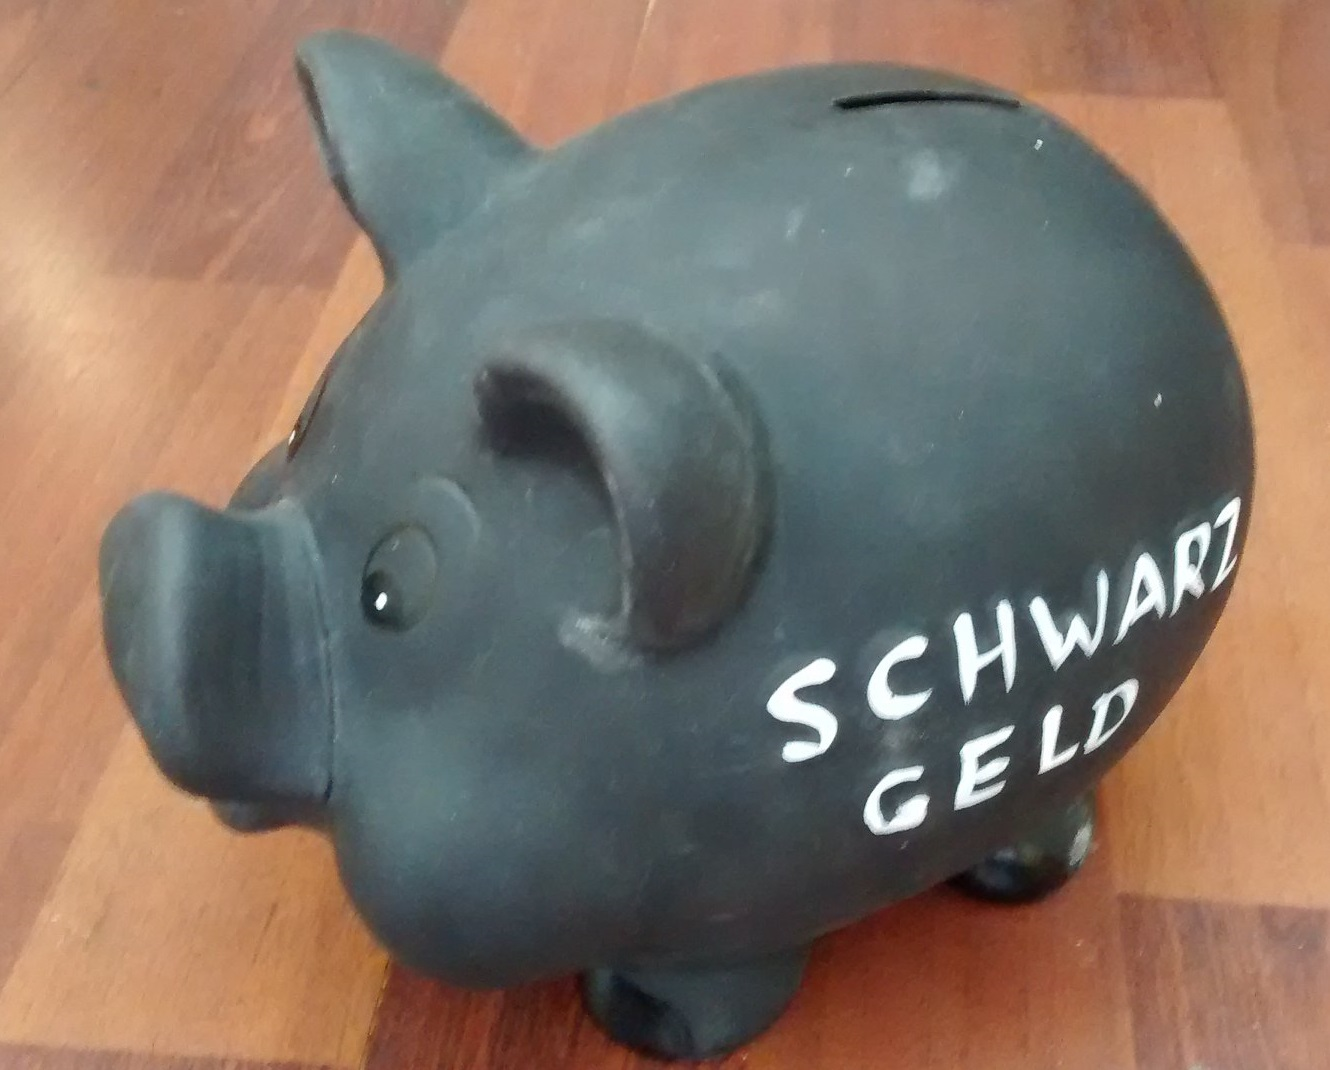
\includegraphics[scale=0.25]{images/sparschwein/photo.jpg}
\label{fig:piggy}
\end{figure}

\section{3D Scanning} % stefan

Die Modelle wurden mit einem Minolta 3D-Scanner virtualisiert. Dabei waren viele Arbeitsschritte bei uns allen ident: Zuerst wurde eine oder mehrere Linsen gewählt, die für den Scannvorgang benutzt werden sollten. Diese Auswahl hing größtenteils von der Größe des Objekts ab, da man den Scanner mit unterschiedlichen Linsen in unterschiedlichen Reichweiten zum Objekt platzieren konnte. Das Objekt selbst wurde auf einen Drehteller platziert, damit automatisch rundum-Messungen vorgenommen werden konnten.

Nachdem man das Objekt gut platziert hatte, musste man den Scanner kalibrieren. Dafür musste man das Objekt wieder vom Drehteller entfernen und stattdessen das Kalibrierungsobjekt in die Mitte des Tellers stellen. Der Scanner nahm dann ein paar Messungen vor und danach war die Kamera zum Drehteller registriert.

Nun konnte man das Objekt wieder auf den Teller platzieren und in der Software einen Autofokus durchführen. Manchmal musste hier der Fokus manuell nachgestellt werden, um eine bessere Tiefenschärfe über das gesamte Objekt zu erlangen. Nachdem nun alles bereit war konnte man den Scanvorgang starten. Der Scanner nahm automatisch 6 Messungen in unterschiedlichen Ansichten vor. Danach konnte das Objekt in eine z.B. liegende Position gebracht werden, um noch eine Messung durchzuführen. Wenn dabei die Kamera und der Drehteller nicht bewegt wurden, musste keine erneute Kalibrierung vorgenommen werden. In Abbildung \ref{fig:scansoftware} kann man einen Screenshot der Software vor einem Scanvorgang sehen.

\begin{figure}[!h]
\caption{Screenshot der Scansoftware vor einem Scanvorgang}
\centering
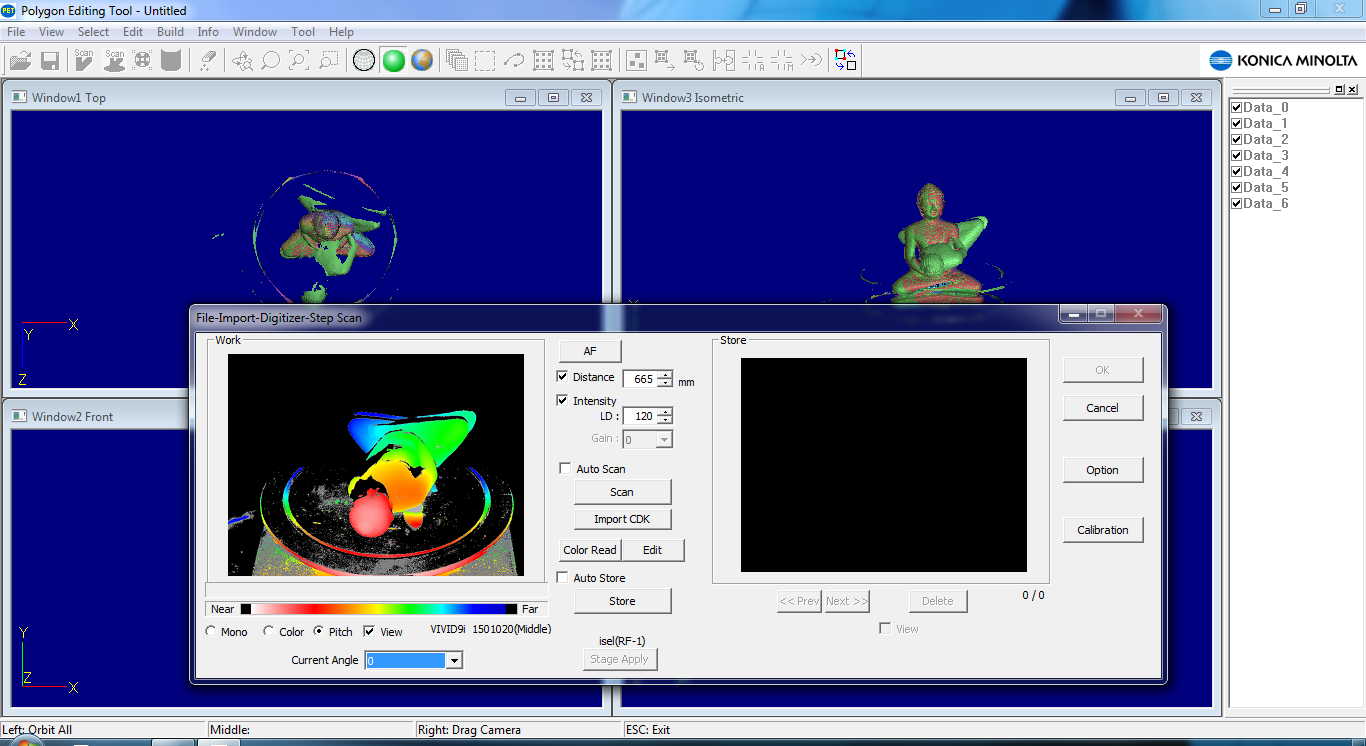
\includegraphics[width=0.9\textwidth]{images/Statue_Liegend.PNG}
\label{fig:scansoftware}
\end{figure}

Nachdem alle Scans vorgenommen wurden mussten die erhobenen Daten nur noch exportiert werden. Diese sind aber keinesfalls schon finalisiert: Zwar sind die Rundumscans innerhalb registriert, doch untereinander noch gar nicht. Manche Scanns wurden in der Software sogar an anderen Orten angezeigt. Um die Daten zu bereinigen, mussten wir zu einer anderen Software greifen: Geomagic Studio.

% Probleme
\subsection{Budha}

Beim Scanvorgang der Budha Statue gab es trotz der dunklen Oberfläche keine nennenswerten Probleme. Auch die leichte Rauheit der Figur führte zu keiner gravierenden Ablenkung der Lasermessung. Für das Gesicht wurde zugunsten einer höheren Genauigkeit auf eine andere Linse zurückgegriffen. Um alle wesentlichen Abschattungen zu scannen wurde die Statue händisch in mehreren Posen aufgestellt um die Armbeuge sowie die Fußleiste der Figur optimal zu erfassen.


\subsection{Mann}
Die Mann-Statuette war ein dankbares Modell. Das Holz war matt genug um keine Probleme zu bereiten und die Form ist annähernd eine Kugel. Nur die Größe war schon grenzwertig. Es ging sich gerade noch aus alle Scans mit einer Linse für Nahaufnahmen durchzuführen. Wäre das Modell ein bisschen größer gewesen, hätten wir die Linse wechseln müssen und dann wäre das Objekt in den Scans sehr klein gewesen.

\subsection{Sparschwein}
Das Sparschwein Modell ist geometrisch nicht komplex, dennoch stellt es für den Minolta 3D-Scanner eine Herausforderung dar. Da das Modell sehr dunkel ist wird  nur ein sehr kleiner Anteil des Laser Lichts reflektiert. Um das zu kompensieren wurde beim Scanvorgang die Intensität des Lasers manuell erhöht. Weiters besitzt das Objekt einige sehr stark reflektierende Teile welche durch den Scanner schlecht bis gar nicht erfasst werden. In den Scans erscheinen diese Bereiche als Löcher. An den reflektierenden Bereichen konnte keine Oberfläche rekonstruiert werden. Glücklicherweise sind diese Bereiche nicht sehr groß und können in der Nachbearbeitung automatisch geschlossen werden.

\section{Nachbearbeitung in Geomagic} % christian

Wie erwartet bestand die Hauptarbeit der Nachbearbeitung der Scandaten. Dabei wurden im wesentlichen folgende Schritte vorgenommen:

\begin{enumerate}
\item Registrierung
\begin{enumerate}
\item Globale Registrierung in Gruppen
\item Manuelle Registrierung der Gruppen, n-Punkt Registrierung
\end{enumerate}
\item Meshgenerierung
\begin{enumerate}
\item Vereinigen der registrierten Meshes
\end{enumerate}
\item Nachbearbeitung
\begin{enumerate}
\item Nachbearbeitung: 2D-Mannigkeitsfehler entfernen, Glätten, Spitzen entfernen, Mesh-Doctor, Löcher füllen
bis modell wasserdicht
\item Feine Nachbearbeitung: Sandpapier
\end{enumerate}
\end{enumerate}

Obwohl die Registrierung von einheitlich erstellten Aufnahmen schon gegeben war, wurde eine globale Registrierung der Scans in den jeweiligen Scangruppen vorgenommen um Fehler weiter zu reduzieren. Zusätzlich erstellte Einzelscans mußten naturgemäß ohnehin in der passenden Gruppe entweder automatisch oder manuell registriert werden.

Die einzelnen Scangruppen wurden anschließend zueinander global registriert, um eine endgültige Ausrichtung der gesammten Range Maps zu erhalten - siehe Abbildung \ref{fig:budhaGlobal}. In vielen Fällen erwies sich eine automatische Registrierung als fehlerhaft bzw. GeoMagic versagte gänzlich den Dienst. Aufgrund dessen wurden viele manuelle Registrierungen aufgrund einer n-Punkt Registration vorgenommen in der Hoffnung dass im Anschluss automatische Registrierungen greifen.

\begin{figure}[H]
\centering
\caption{Globale Registrierung - Falschfarbendarstellung der verschiedenen Range Maps}
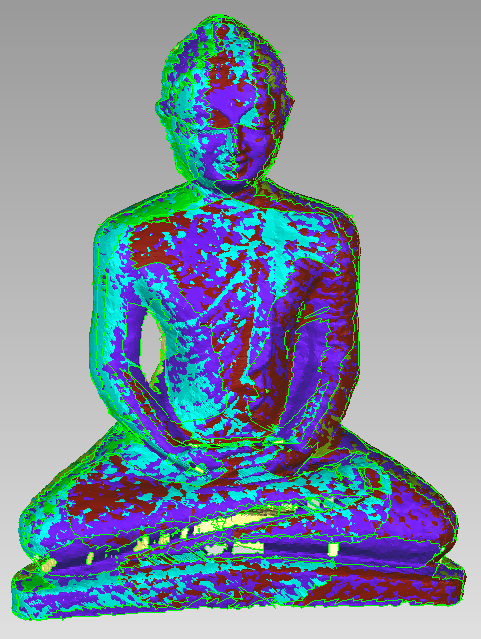
\includegraphics[scale=0.35]{images/GeoMagicBudhaPictures/Budha_Scans_Aufrecht_globalRegistration_2.PNG}
\label{fig:budhaGlobal}
\end{figure}

Bei der n-Punkt Registration wurden fixe und bewegliche Scans zueinander definiert und identische Punkte an der Oberfläche für die Registrierung definiert. Dabei war darauf zu achten, dass die Punkte möglichst großflächig und nicht auf einer Linie bzw. in einer Ebene zueinander liegen damit eine möglichst gute Annäherung sicher gestellt werden konnte - siehe Abbildung \ref{fig:budhaManual}. Aus den Range Maps wurden auch fehlerhafte Bereiche, insbesondere an den Rändern der Scans entfernt. Eine (erneute) Registrierung auf dieser Basis brachte eine weitere Verbesserung der Annäherung auf den bereinigten Daten mit sich.

\begin{figure}[H]
\caption{Manuelle n-Punkt Registrierung}
\centering
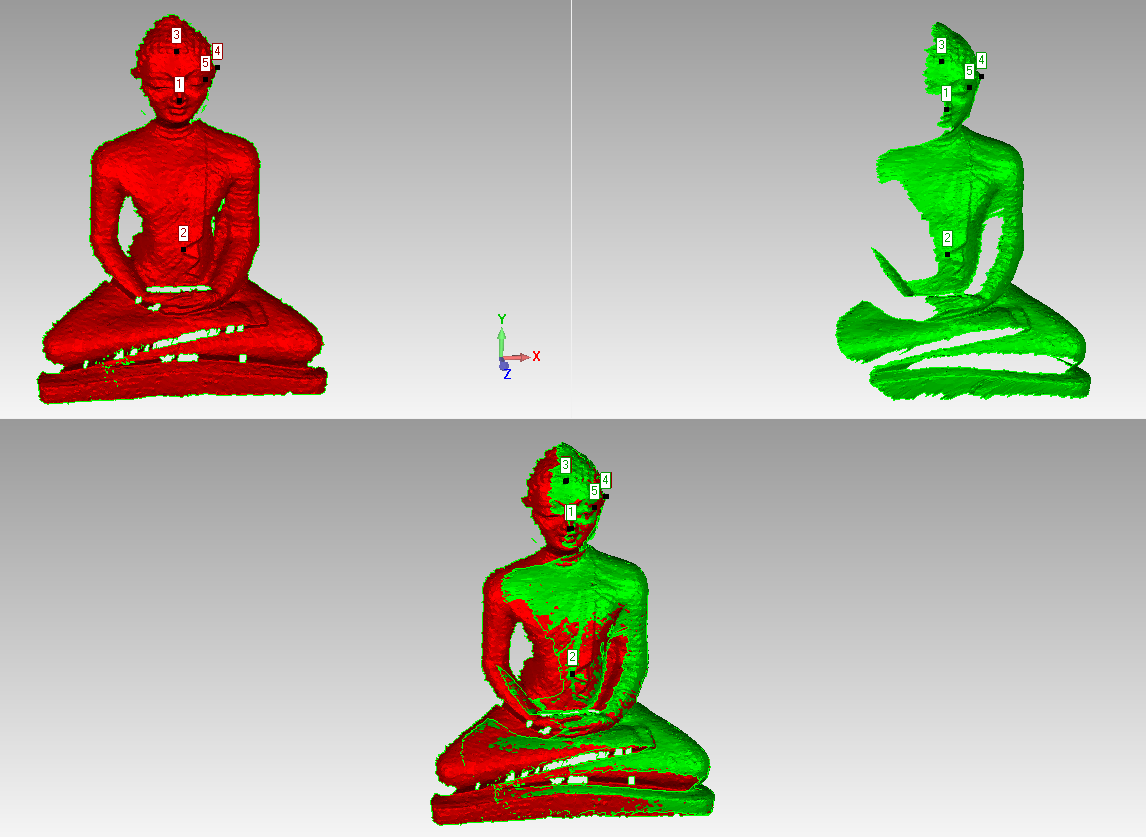
\includegraphics[scale=0.35]{images/GeoMagicBudhaPictures/Budha_Scans_Aufrecht_manualRegistration_03.PNG}
\label{fig:budhaManual}
\end{figure}
 
Vor der Vereinigung der Meshes wurden noch die Teilmeshes auf ein vernünftiges Maß an Polygonen reduziert, um in vertretbarer Zeit auf ein brauchbares Ergebnis zu kommen.
Nach der Vereinigung mußte der resultierende Mesh weitere Bearbeitungsschritte durchwandern. Der Mesh-Doktor von GeoMagic lieferte dabei gute Dienste - siehe Abbildung \ref{fig:budhaMeshDoc}. Die aufgeführten Identifizierungen zeigten:

\begin{itemize}
\item nicht-mannigfaltige Kanten
\item Selbstüberschneidungen
\item extreme Kantenwinkel
\item Spikes
\item Kleine Komponenten
\item Kleine Tunnel
\item Kleine Löcher
\end{itemize}

\begin{figure}[H]
\caption{Mesh-Doktor - Highlighting von defekten oder zu bearbeitenden Stellen}
\centering
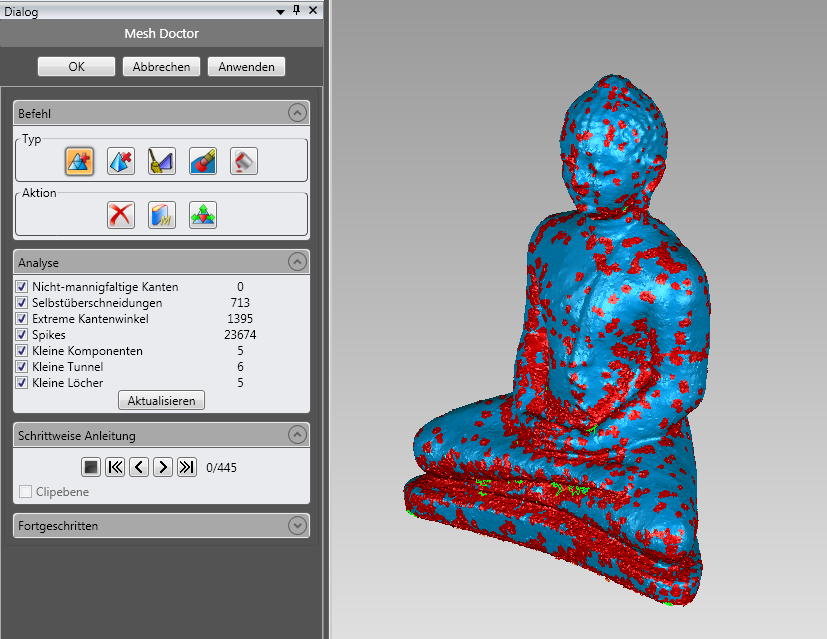
\includegraphics[scale=0.35]{images/GeoMagicBudhaPictures/Budha_MeshDoctor.PNG}
\label{fig:budhaMeshDoc}
\end{figure}

Teilweise wurde die automatische Reparatur bzw. Bereinigung angewandt, teilweise diente der Mesh-Doktor als Guide für manuelle Anpassungen im Mesh, insbesondere von Löschen fehlerhafter Geometrie und erneuter Rekonstruktion aus dem Umfeld. Diese manuelle Bearbeitung der teilweise künstlich eingeführten oder erweiterten Löcher wird exemplarisch am Schließen eines Loches in der Grundfläche einer Figur demonstriert - siehe Tabelle \ref{tab:BudhaHole}.

\begin{table}[h]
	\caption{Manuelles Schließen der Grundfläche einer Figur, links vorher, rechts nachher}
	\begin{center}
		\begin{tabular}{| c | c |}
			\hline
			\multicolumn{2}{|l|}{
				\begin{tabular}{ l }
				\emph{Budha - manuelles Schließen} \\
				\end{tabular}
			} \\
			\hline
			offen & geschlossen \\
			\hline
			\hline
			& \\
			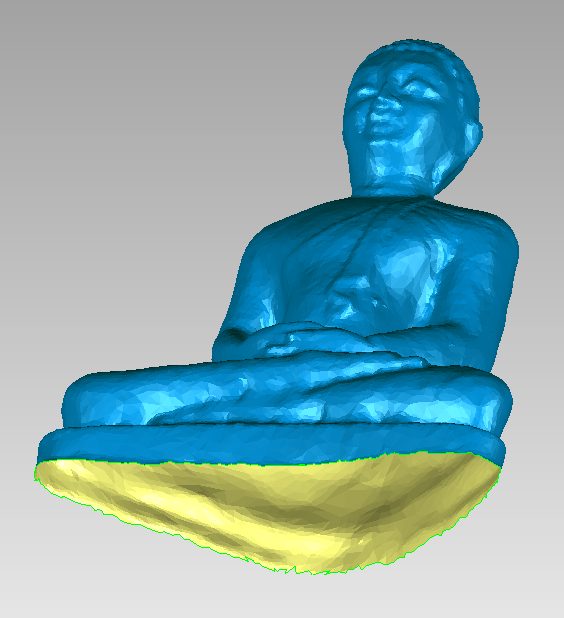
\includegraphics[width=0.45\textwidth]{./Images/GeomagicBudhaPictures/Budha_SfM_BottomHole_2.PNG} & 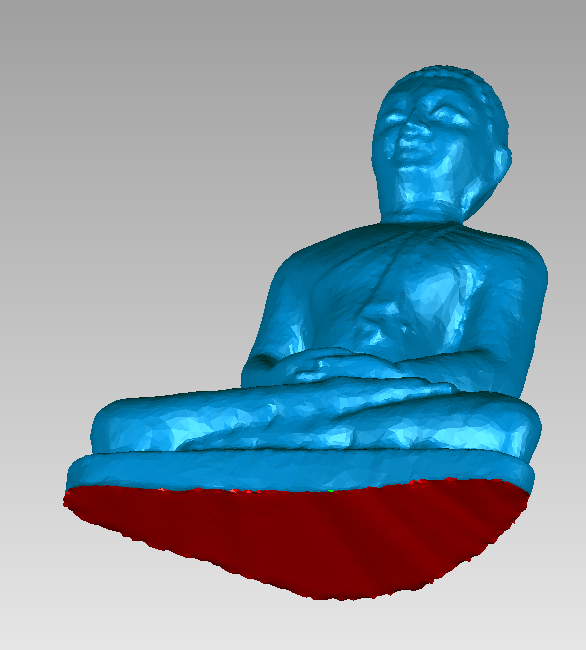
\includegraphics[width=0.45\textwidth]{./Images/GeomagicBudhaPictures/Budha_SfM_BottomHoleClosed_2.PNG} \\
			\hline					  
		\end{tabular}
	\end{center}
	\label{tab:BudhaHole}
\end{table}

Schlußendlich wurden noch Bearbeitungen wie  Glätten und Sandpapierbearbeitungen an bestimmten Stellen vorgenommen um den Gesamteindruck der Figur zu verbessern - siehe Tabelle \ref{tab:BudhaSmooth}.

\begin{table}[h]
	\caption{Manuelles Glätten einer Figur, links vorher, rechts nachher}
	\begin{center}
		\begin{tabular}{| c | c |}
			\hline
			\multicolumn{2}{|l|}{
				\begin{tabular}{ l }
				\emph{Budha - manuelles Glätten} \\
				\end{tabular}
			} \\
			\hline
			vor Glättung & nach Glättung \\
			\hline
			\hline
			& \\
			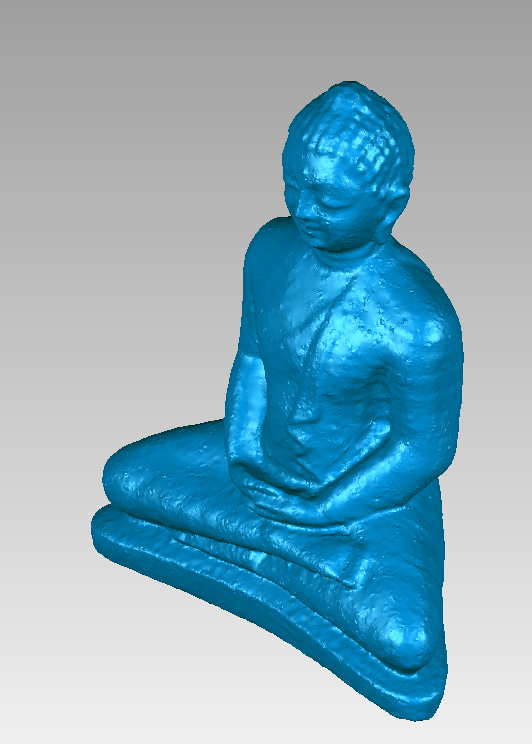
\includegraphics[width=0.45\textwidth]{./Images/GeomagicBudhaPictures/Budha_Presmooth.PNG} & 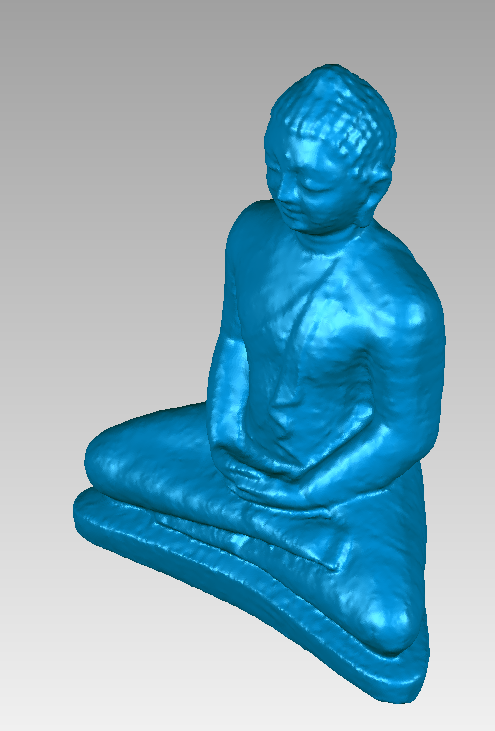
\includegraphics[width=0.43\textwidth]{./Images/GeomagicBudhaPictures/Budha_Postsmooth.PNG} \\
			\hline					  
		\end{tabular}
	\end{center}
	\label{tab:BudhaSmooth}
\end{table}

\subsection{Waterproof 3D Model}

Das Schließen des Modells erforderte manuelle Arbeit für jedes einzelne Loch. Das beste Vorgehen bestand darin, die Umgebung des Loches von von allen störenden Artefakten zu befreien welche die 2D Mannigfaltigkeit des Meshes in diesem Bereich stören. Danach wird das Loch unter Berücksichtigung der Krümmung der umgebenden Oberfläche geschlossen.

% Nachbearbeitung und Probleme
\subsection{Budha}

Zunächst wurden alle $40$ Scans gruppiert und manuell in den Gruppen zueinander registriert, da eine automatische Registrierung in den meisten Fällen fehlschlug.

Danach wurden die einzelnen Gruppen zueinander registriert um eine Gesamtdatenbasis des Modells zu erhalten.

Im Anschluss wurden auf den einzelnen Scans Fehler an den Scanrändern und bzw. überflüssige Teile der Scans von der Scanplatte entfernt.

Eine erneute Registrierung der bereinigten Daten verbesserte die Passgenauigkeit etwas. 
Auch wurden die Meshes dezimiert, damit die Datenmenge handhabbarer wurde als auch der Resultat des Merge-Vorgangs deutlich verbesserte.

Das Merging wurde auf Basis von allen Scans und auf Basis einer reduzierten Anzahl von Scans vorgenommen um Überlagerungen von identischen Scandaten zu vermeiden.

In der Reduktion wurde auf die detailierten Facescans und auf die doppelt vorhandenen 360 Grad Scans der aufrechten Figur zugunsten eines besseren Rausch- bzw. Interpolationsverhaltens verzichtet.


\subsection{Mann}
Bei der Nachbearbeitung habe ich einen großen Fehler begangen: ich habe sehr lange Zeit nicht gespeichert, ganz und gar darauf vergessen. Nachdem ich das Objekt vereinigt hatte, stürzte die Software ab und ich musste alles noch einmal machen. Dieser Fehler ist mir dann nicht mehr unterlaufen. Ansonsten bin ich auf keine besonderen Probleme gestoßen.

\subsection{Sparschwein}
Durch die einfache Geometrie des Modells war auch die Nachbearbeitung der Oberfläche relativ einfach. Fast alle Bereiche der Oberfläche weisen eine sehr niedrige Krümmung auf. Dadurch hatte das rekonstruierte Modell auch schon vor der Nachbearbeitung nur sehr wenige Fehler. Am meisten Probleme bereitete der Münzeinwurfschlitz. Da die Hülle des Sparschweins nur wenige Millimeter dick ist wurde innerhalb des Schlitzes keine Geometrie aufgenommen. Ein automatisches Schließen des Bereiches hat erst nach einigen Versuchen zum gewünschten Ergebnis geführt, da je nach dem wie viel Geometrie gelöscht wurde sich auch die automatische Rekonstruktion verändert. 

\section{Evaluierung}
Um die Qualität der 3D-Scans zu beurteilen wurden Messungen an den realen Objekten durchgeführt und mit Messungen an den erzeugten Modellen verglichen.

% Messungen
\subsection{Budha}

Aufgrund der Tatsache dass Geomagic die beiden 3D-Modelle des 3D-Scans und der SfM-Erfassung leider nicht per Registrierung aneinander ausrichten konnte wurde aufgrund von optischer Übereinstimmung eine Skalierung und Überlagerung der Modelle per Hand vorgenommen. Da insbesondere die Höhe der Fußleiste im SfM-Modell eher auf einer begründeten Schätzung basiert ist es nicht verwunderlich, dass große Fehler in der Volumensbestimmung zu erwarten waren. Die Berechnung des Volumens der beiden Modelle basiert auf folgender gezeigten händischen Überlagerung \ref{fig:budhaMerge}.

\begin{figure}[H]
\caption{Budha}
\centering
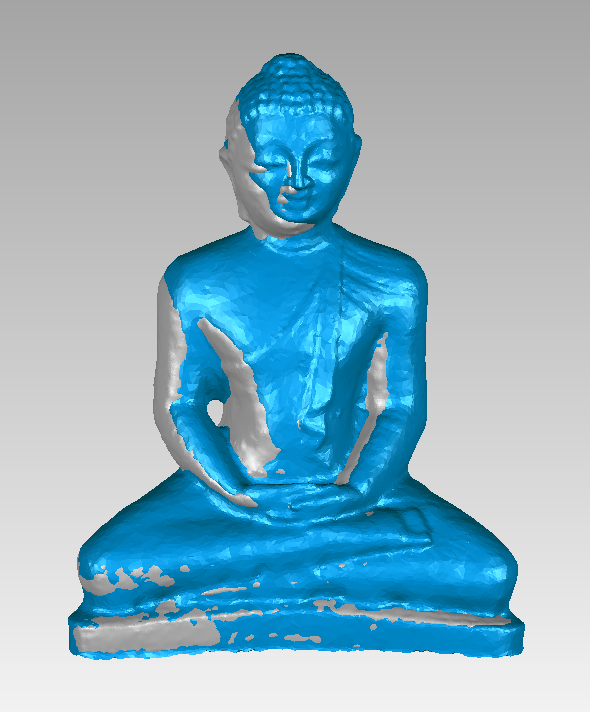
\includegraphics[scale=0.4]{images/GeoMagicBudhaPictures/Budha_Merge_SfM_3DScan.PNG}
\label{fig:budhaMerge}
\end{figure}

Der Volumensvergleich von dem 3D-Scan-Modell zu dem SfM-Modell beträgt $204007 mm^3$ zu $214291 mm^3$, relativ also $5 \%$ Unterschied. 

\subsection{Mann}
Beim Mann wurden beim Vergleich der Messungen des Originals gegen die Minolta-Scans von rund $\pm 0.9$mm festgestellt(Siehe Tabelle \ref{tab:man:errorScan}). Das Volumen des Originalmodells konnte nicht ermittelt werden, da Wasser die Figur geschädigt hätte. Das von Geomagic berechnete Volumen beträgt $544250.14mm^3$.

\begin{table}[h!]
\centering
\begin{tabular}{l | c c | c}
Modell: Mann& Original & Scan & Diff\\
\hline
Fußlänge & $34.76$mm & $35.94$mm & $-1.18$mm\\
Armlänge & $70.53$mm & $69.80$mm & $0.73$mm\\
Hosenbund & $14.95$mm & $15.83$mm & $0.88$mm\\
\hline \hline
Durchschnitt & & & $\pm 0.93$mm
\end{tabular}
\caption{Messfehler Original/Minolta-Scan}
\label{tab:man:errorScan}
\end{table}

\subsection{Sparschwein}
Für das Sparschwein wurden 7 Messungen an markanten Punkten durchgeführt. Ein Vergleich der Messungen am Modell mit Messungen am realen Objekt ließ eine Genauigkeit von $\pm 1$mm feststellen. Da das Objekt hohl ist konnte das Volumen leider nicht ermittelt werden.

\section{Structure from Motion mit 123d Catch} % dominik

Autodesk 123d Catch ist eine Online Platform für Structure from Motion rekonstruktion. Zunächst werden Bilder des Objektes in konzentrischen Kreisen und aus mehreren Winkeln aufgenommen. Dabei ist es wichtig für eine gleichbleibende Beleuchtung zu sorgen. Am besten verwendet man mehrere Lampen die das Objekt gleichmäßig ausleuchten. Beim Aufnehmen der Bilder muss man sehr darauf achten keine Schatten auf das Objekt zu werfen. Nachdem man ~40+ Bilder aufgenommmen hat werden diese mit der 123d Catch Applikation hochgeladen und automatisch verarbeitet. Sobald der Vorgang abgeschlossen ist kann man das fertige Modell herunterladen. Die Rekonstruktion nimmt mit einer Berechnungszeit von ca. 45 Minuten sehr viel Zeit in Anspruch da die gesamte Verarbeitung der Daten am Server passiert. Ein großer Vorteil der Technologie ist dass keine spezielle Hardware benötigt wird. Sogar eine Handykamera reicht bereits aus um gute Ergebnisse zu erzielen.

% Vergleich der einzelnen Modelle
\subsection{Budha}

Die Aufnahmen für den Budha wurden unter diffusem Tageslicht mit Deckenbeleuchtung und einem Spot von oben vorgenommen. Dadurch war die Beleuchtung konstant und aufgrund der Profilierung und der Grauwertunterschiede auf der Steinstruktur konnten ausreichend Features zu einer gelungenen Rekonstruktion ermittelt werden. Die Aufnahmen geschahen in drei konzentrischen Kreisen in verschiedener Höhe um die Figur plus zwei Aufnahmen von oben.
Nur in der Armbeuge gab es wie erwartet Probleme, ebenfalls in der Abgrenzung der Figur zum Untergrund. Ansonsten stellte die Rekonstruktion eine gute Annäherung der Figur dar - siehe Tabelle \ref{tab:Budha-SfM}.

\begin{table}[h]
	\caption{Darstellung der Budha-Figur aus der Structure from Motion Rekonstruktion. Linke Darstellung texturiert, rechte Darstellung untexturiert.}
	\begin{center}
		\begin{tabular}{| c | c |}
			\hline
			\multicolumn{2}{|l|}{
				\begin{tabular}{ l }
				\emph{Budha SfM Rekonstruktion} \\
				\end{tabular}
			} \\
			\hline
			texturiert & untexturiert \\
			\hline
			\hline
			 & \\
			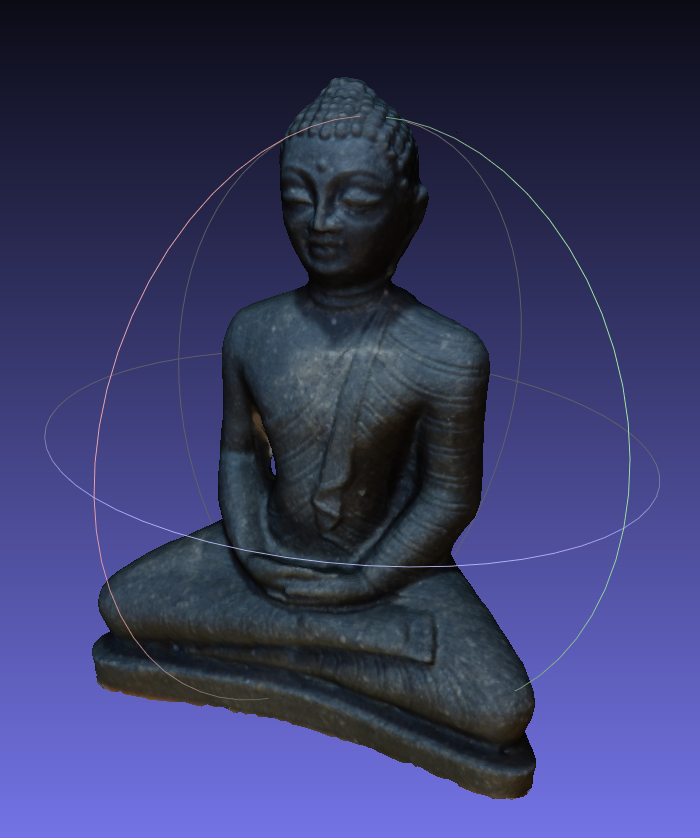
\includegraphics[width=0.45\textwidth]{./Images/Budha/Budha_SfM_Textured.png} & 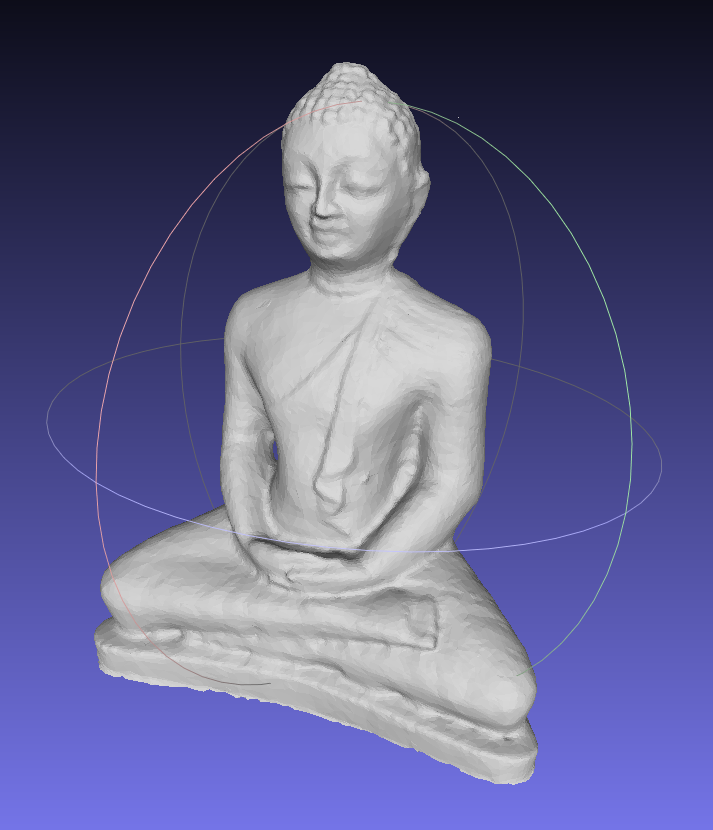
\includegraphics[width=0.46\textwidth]{./Images/Budha/Budha_SfM_Untextured.png} \\
			\hline
			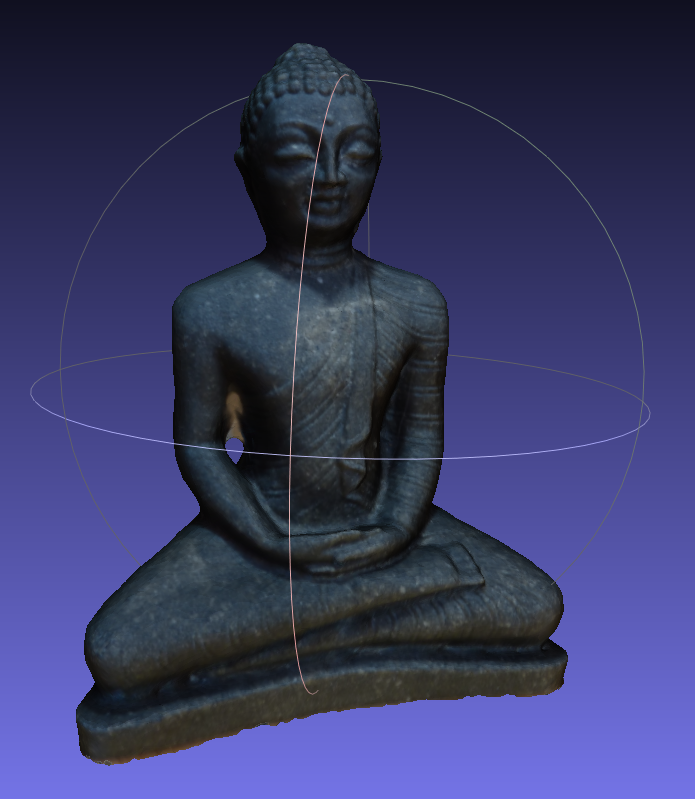
\includegraphics[width=0.48\textwidth]{./Images/Budha/Budha_SfM_Textured_2.png} & 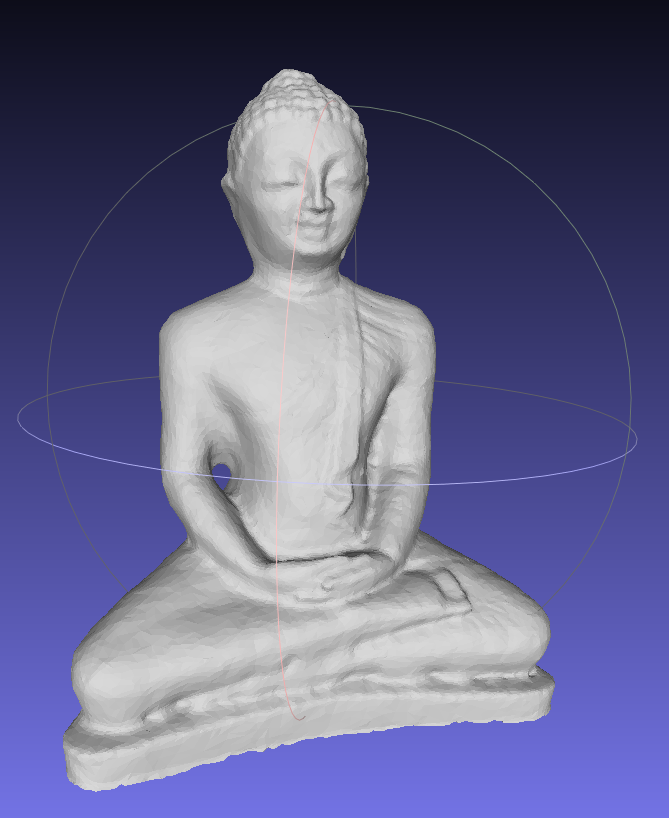
\includegraphics[width=0.45\textwidth]{./Images/Budha/Budha_SfM_Untextured_2.png} \\
			\hline					  
		\end{tabular}
	\end{center}
	\label{tab:Budha-SfM}
\end{table}

\subsection{Mann}
Erwartungsgemäß ist das Modell, das mit 123D Catch erstellt worden ist weniger akkurat als jenes, das mit dem Laserscanner vermessen wurde. Dennoch weist das Modell einen hohen Detail und Genauigkeitsgrad auf. Zwar war eine direkte Messung nicht möglich, da bei Structure from Motion Algorithmen nur relative Werte entstehen, aber nachdem ich das Modell in Geomagic so gut wie möglich an den Minolta Scan angenähert hatte, konnte ich die Messungen durchführen.

Man kann allerdings auch mit dem freien Auge erkennen, dass der Rücken der Statue nicht gut erkannt wurde. Der Hosenbund, der auf dem Original sehr deutlich zu erkennen ist verschwimmt bei der Rekonstruktion mit dem Rücken. Das kann man dadurch erklären, dass der Rücken bei der Aufnahme von der Lichtquelle abgewandt war und deshalb nicht genügend Features gefunden werden konnten.

Beim Mann wurden beim Vergleich der Messungen des Originals gegen die Rekonstruktion von 123d Catch von rund $\pm 2.6$mm festgestellt(Siehe Tabelle \ref{tab:man:errorSFM}). Das von Geomagic berechnete Volumen beträgt $583912.27mm^3$, das ist ein Unterschied von $39662.13mm^3(7.28\%)$ zum Minolta-Scan.

\begin{table}[h!]
\centering
\begin{tabular}{l | c c | c}
Modell: Mann& Original & SFM & Diff\\
\hline
Fußlänge & $34.76$mm & $38$mm & $-3.24$mm\\
Armlänge & $70.53$mm & $73.07$mm & $-2.54$mm\\
Hosenbund & $14.95$mm & $12.88$mm & $2.07$mm\\
\hline \hline
Durchschnitt & & & $\pm 2.62$mm
\end{tabular}
\caption{Messfehler Original/123D Catch}
\label{tab:man:errorSFM}
\end{table}

\begin{figure}[hbtp]
\caption{Vergleich Scan vs 123D Catch}

\begin{subfigure}{\textwidth}
	\caption{Ansicht von Vorne(Scan rechts, 123D Catch links)}
	\centering
	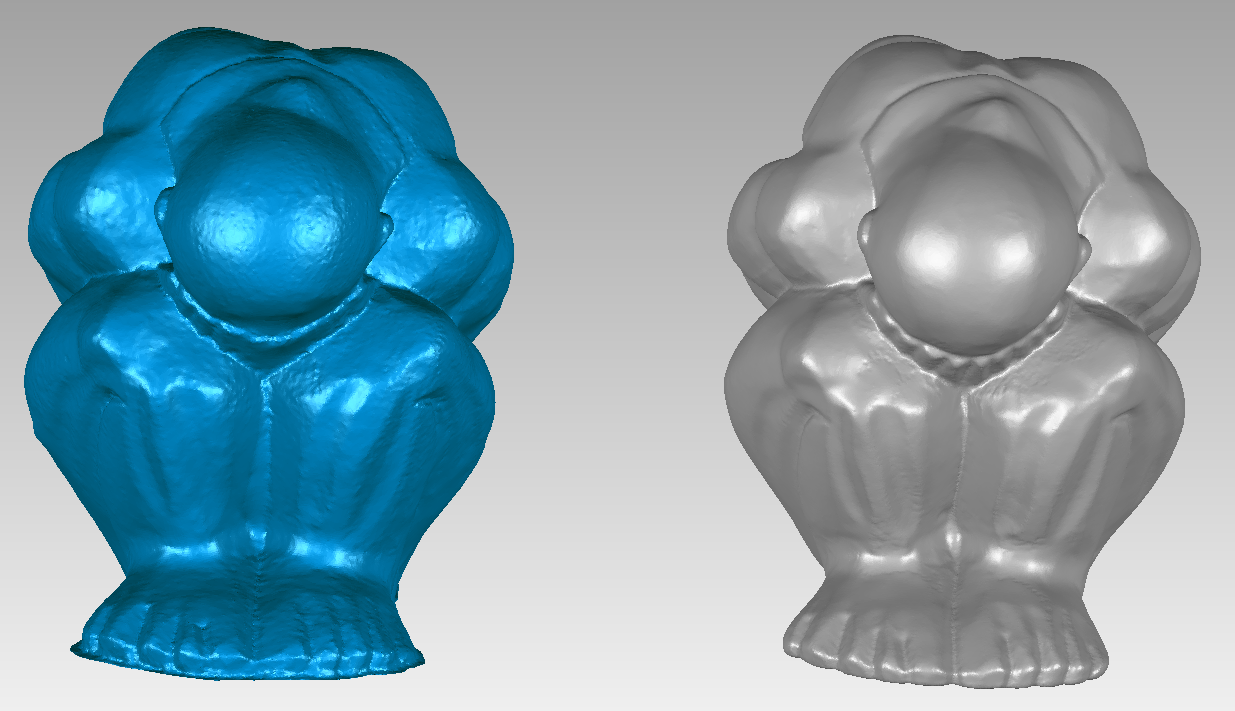
\includegraphics[width=\textwidth]{images/Mann_20_Comparison_Front.PNG}
\end{subfigure}

\begin{subfigure}{\textwidth}
	\caption{Ansicht von Hinten(Scan links, 123D Catch rechts)}
	\centering
	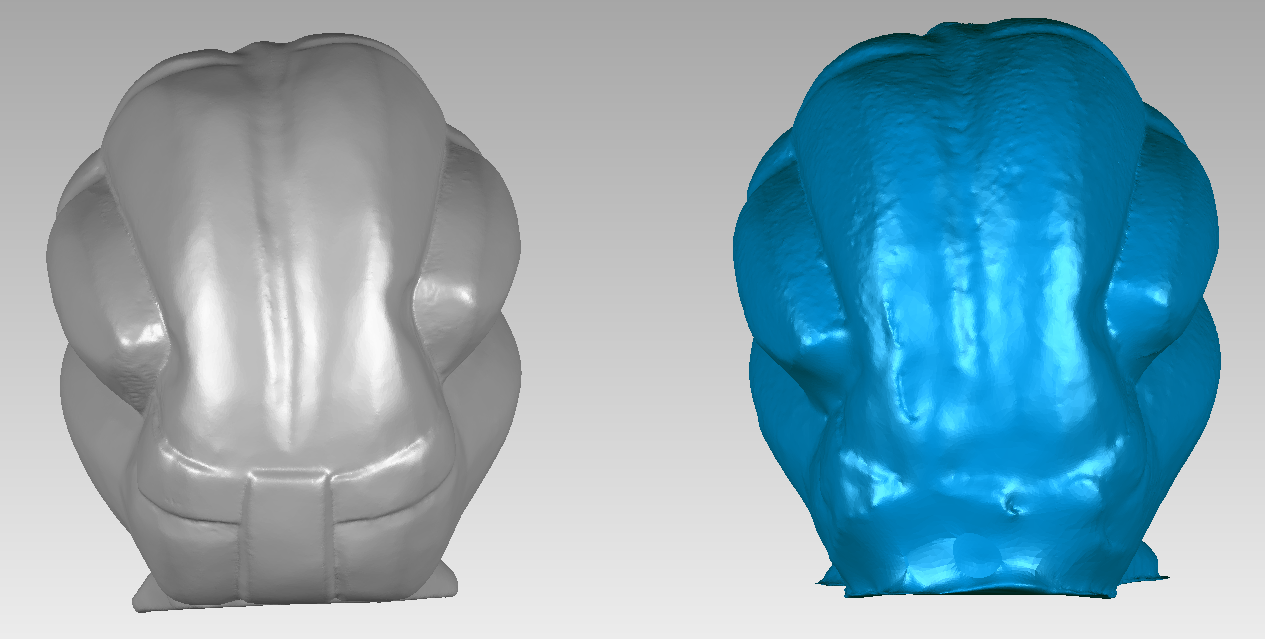
\includegraphics[width=\textwidth]{images/Mann_19_Comparison_Back.PNG}
\end{subfigure}

\end{figure}

\subsection{Sparschwein}
Im Gegensatz zum Laserscanner hat 123d Catch große Probleme das Sparschwein zu rekonstruieren. Die Structure from Motion Technik verwendet Bildfeatures um die Bilder zueinander zu registrieren. Leider hat das Modell aber nur sehr wenige verwendbare Features. Entsprechend schlecht fällt das Ergebnis aus. In einem ersten Versuch wurden die Bilder so aufgenommen dass das Sparschwein das ganze Bild ausfüllt. In diesem Fall konnte 123d Catch überhaupt keine Registrierung erreichen. Um die Bilder mit Features anzureichern wurden die Aufnahmen in weiteren Versuchen aus etwas größerer Entfernung aufgenommen. Dadurch konnte 123d Catch die Bilder ohne manuelle Registrierung verarbeiten. Das Ergebnis war aber noch unbefriedigend. 
Für eine bessere Rekonstruktion hab ich dann das Objekt wieder bildfüllend aufgenommen und ca. 20 der 40 Bilder manuell registriert. Das Ergebnis ist in 
Abbildung\ref{fig:piggy_vergleich} zu sehen.

\begin{figure}[p]
\caption{Vergleich Sparschwein Minolta / 123d catch}
\centering
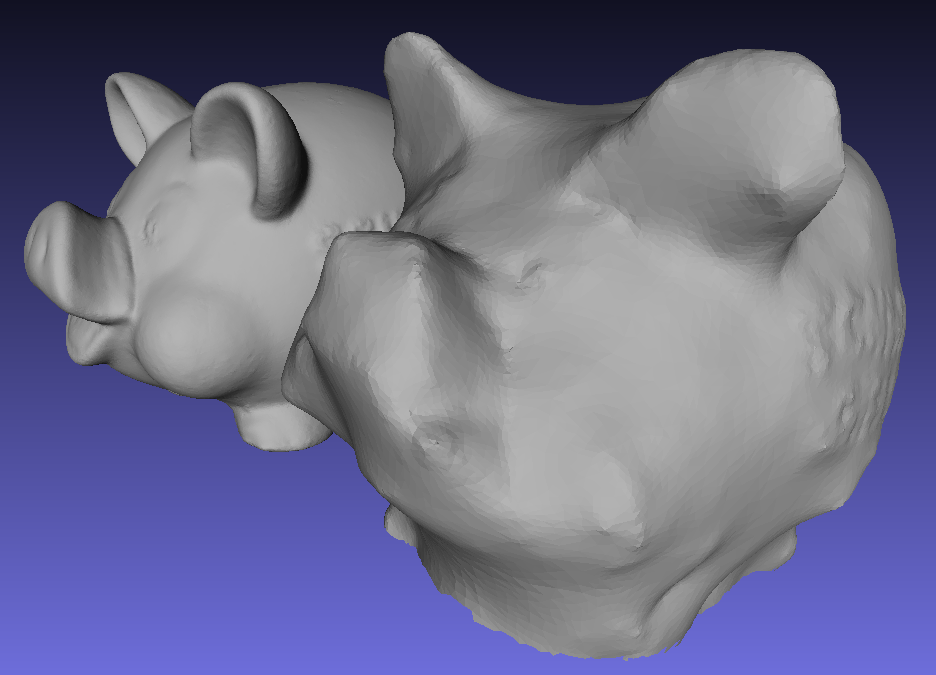
\includegraphics[width=80mm]{images/sparschwein/123d_Vergleich} % ersetzen
\label{fig:piggy_vergleich}
\end{figure}

\begin{figure}[p]
\caption{Sparschwein 123d catch texturiert}
\centering
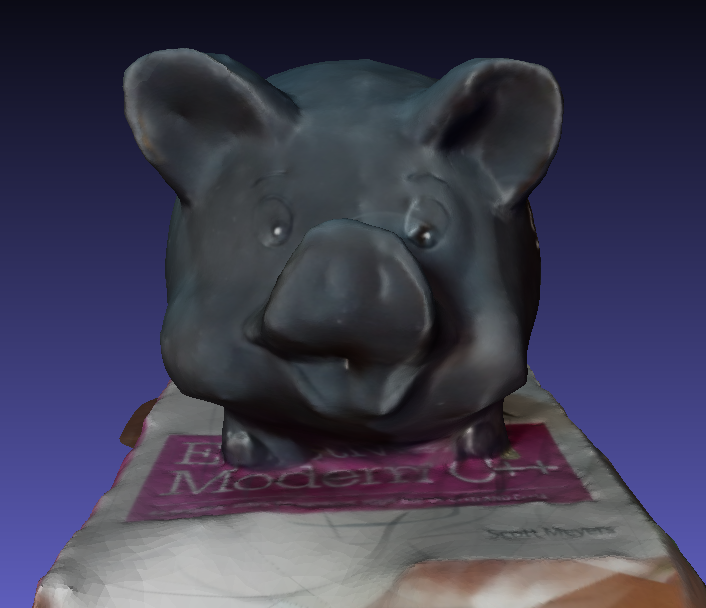
\includegraphics[width=80mm]{images/sparschwein/123d_Texture} % ersetzen
\end{figure}

\begin{figure}[p]
\centering
\caption{Sparschwein finales Modell}
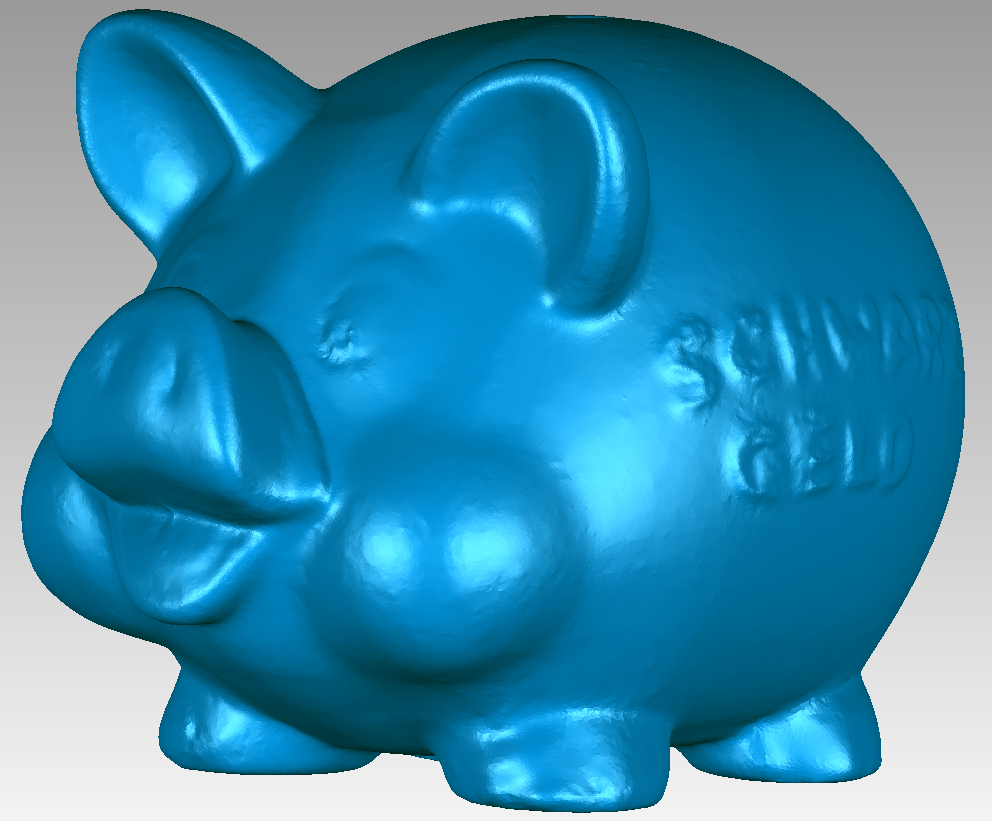
\includegraphics[width=80mm]{images/sparschwein/final} % ersetzen}
\end{figure}
		
\end{document}
